\documentclass{standalone}
\usepackage{tikz}
\usepackage{pgfplots}
\begin{document}
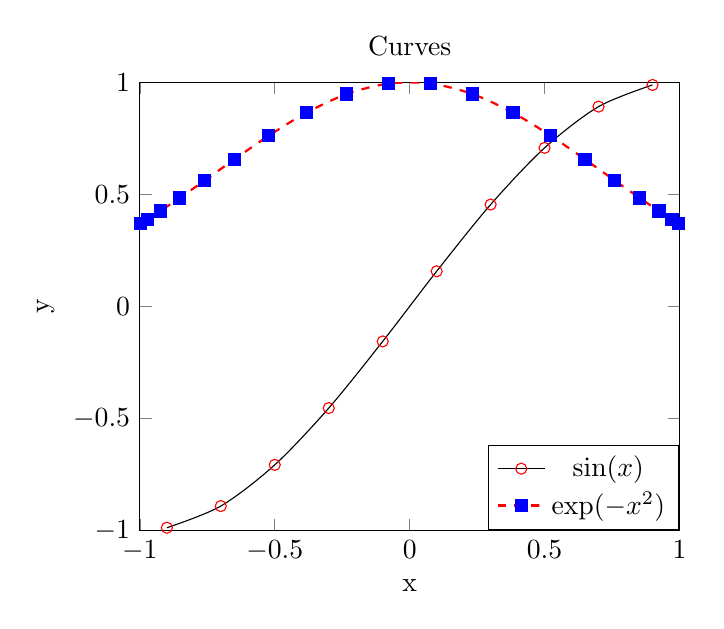
\begin{tikzpicture}
\begin{axis}[
title = Curves,
xlabel = {x},
ylabel = {y},
xmin	= -1, xmax = 1,
ymin	= -1, ymax = 1,
legend style ={
at={(1, 0)},
anchor = south east
}
]
\addplot[
black,
thin,
,
smooth,
mark = o,
mark options = {red, solid,},
] coordinates {
	(-0.9,-0.987688)
	(-0.7,-0.891007)
	(-0.5,-0.707107)
	(-0.3,-0.45399)
	(-0.1,-0.156434)
	(0.1,0.156434)
	(0.3,0.45399)
	(0.5,0.707107)
	(0.7,0.891007)
	(0.9,0.987688)
};
\addplot[
red,
dashed,
thick,
smooth,
mark = square*,
mark options = {blue, solid,},
] coordinates {
	(0.996917,0.370151)
	(0.97237,0.388484)
	(0.92388,0.425899)
	(0.85264,0.483359)
	(0.760406,0.560897)
	(0.649448,0.655877)
	(0.522499,0.761089)
	(0.382683,0.863772)
	(0.233445,0.946962)
	(0.0784591,0.993863)
	(-0.0784591,0.993863)
	(-0.233445,0.946962)
	(-0.382683,0.863772)
	(-0.522499,0.761089)
	(-0.649448,0.655877)
	(-0.760406,0.560897)
	(-0.85264,0.483359)
	(-0.92388,0.425899)
	(-0.97237,0.388484)
	(-0.996917,0.370151)
};
\legend{$\sin(x)$, $\exp(-x^2)$};
\end{axis}
\end{tikzpicture}
\end{document}
